\section{Fazit}\label{sec:fazit}
\begin{figure}[H]
  \centering
  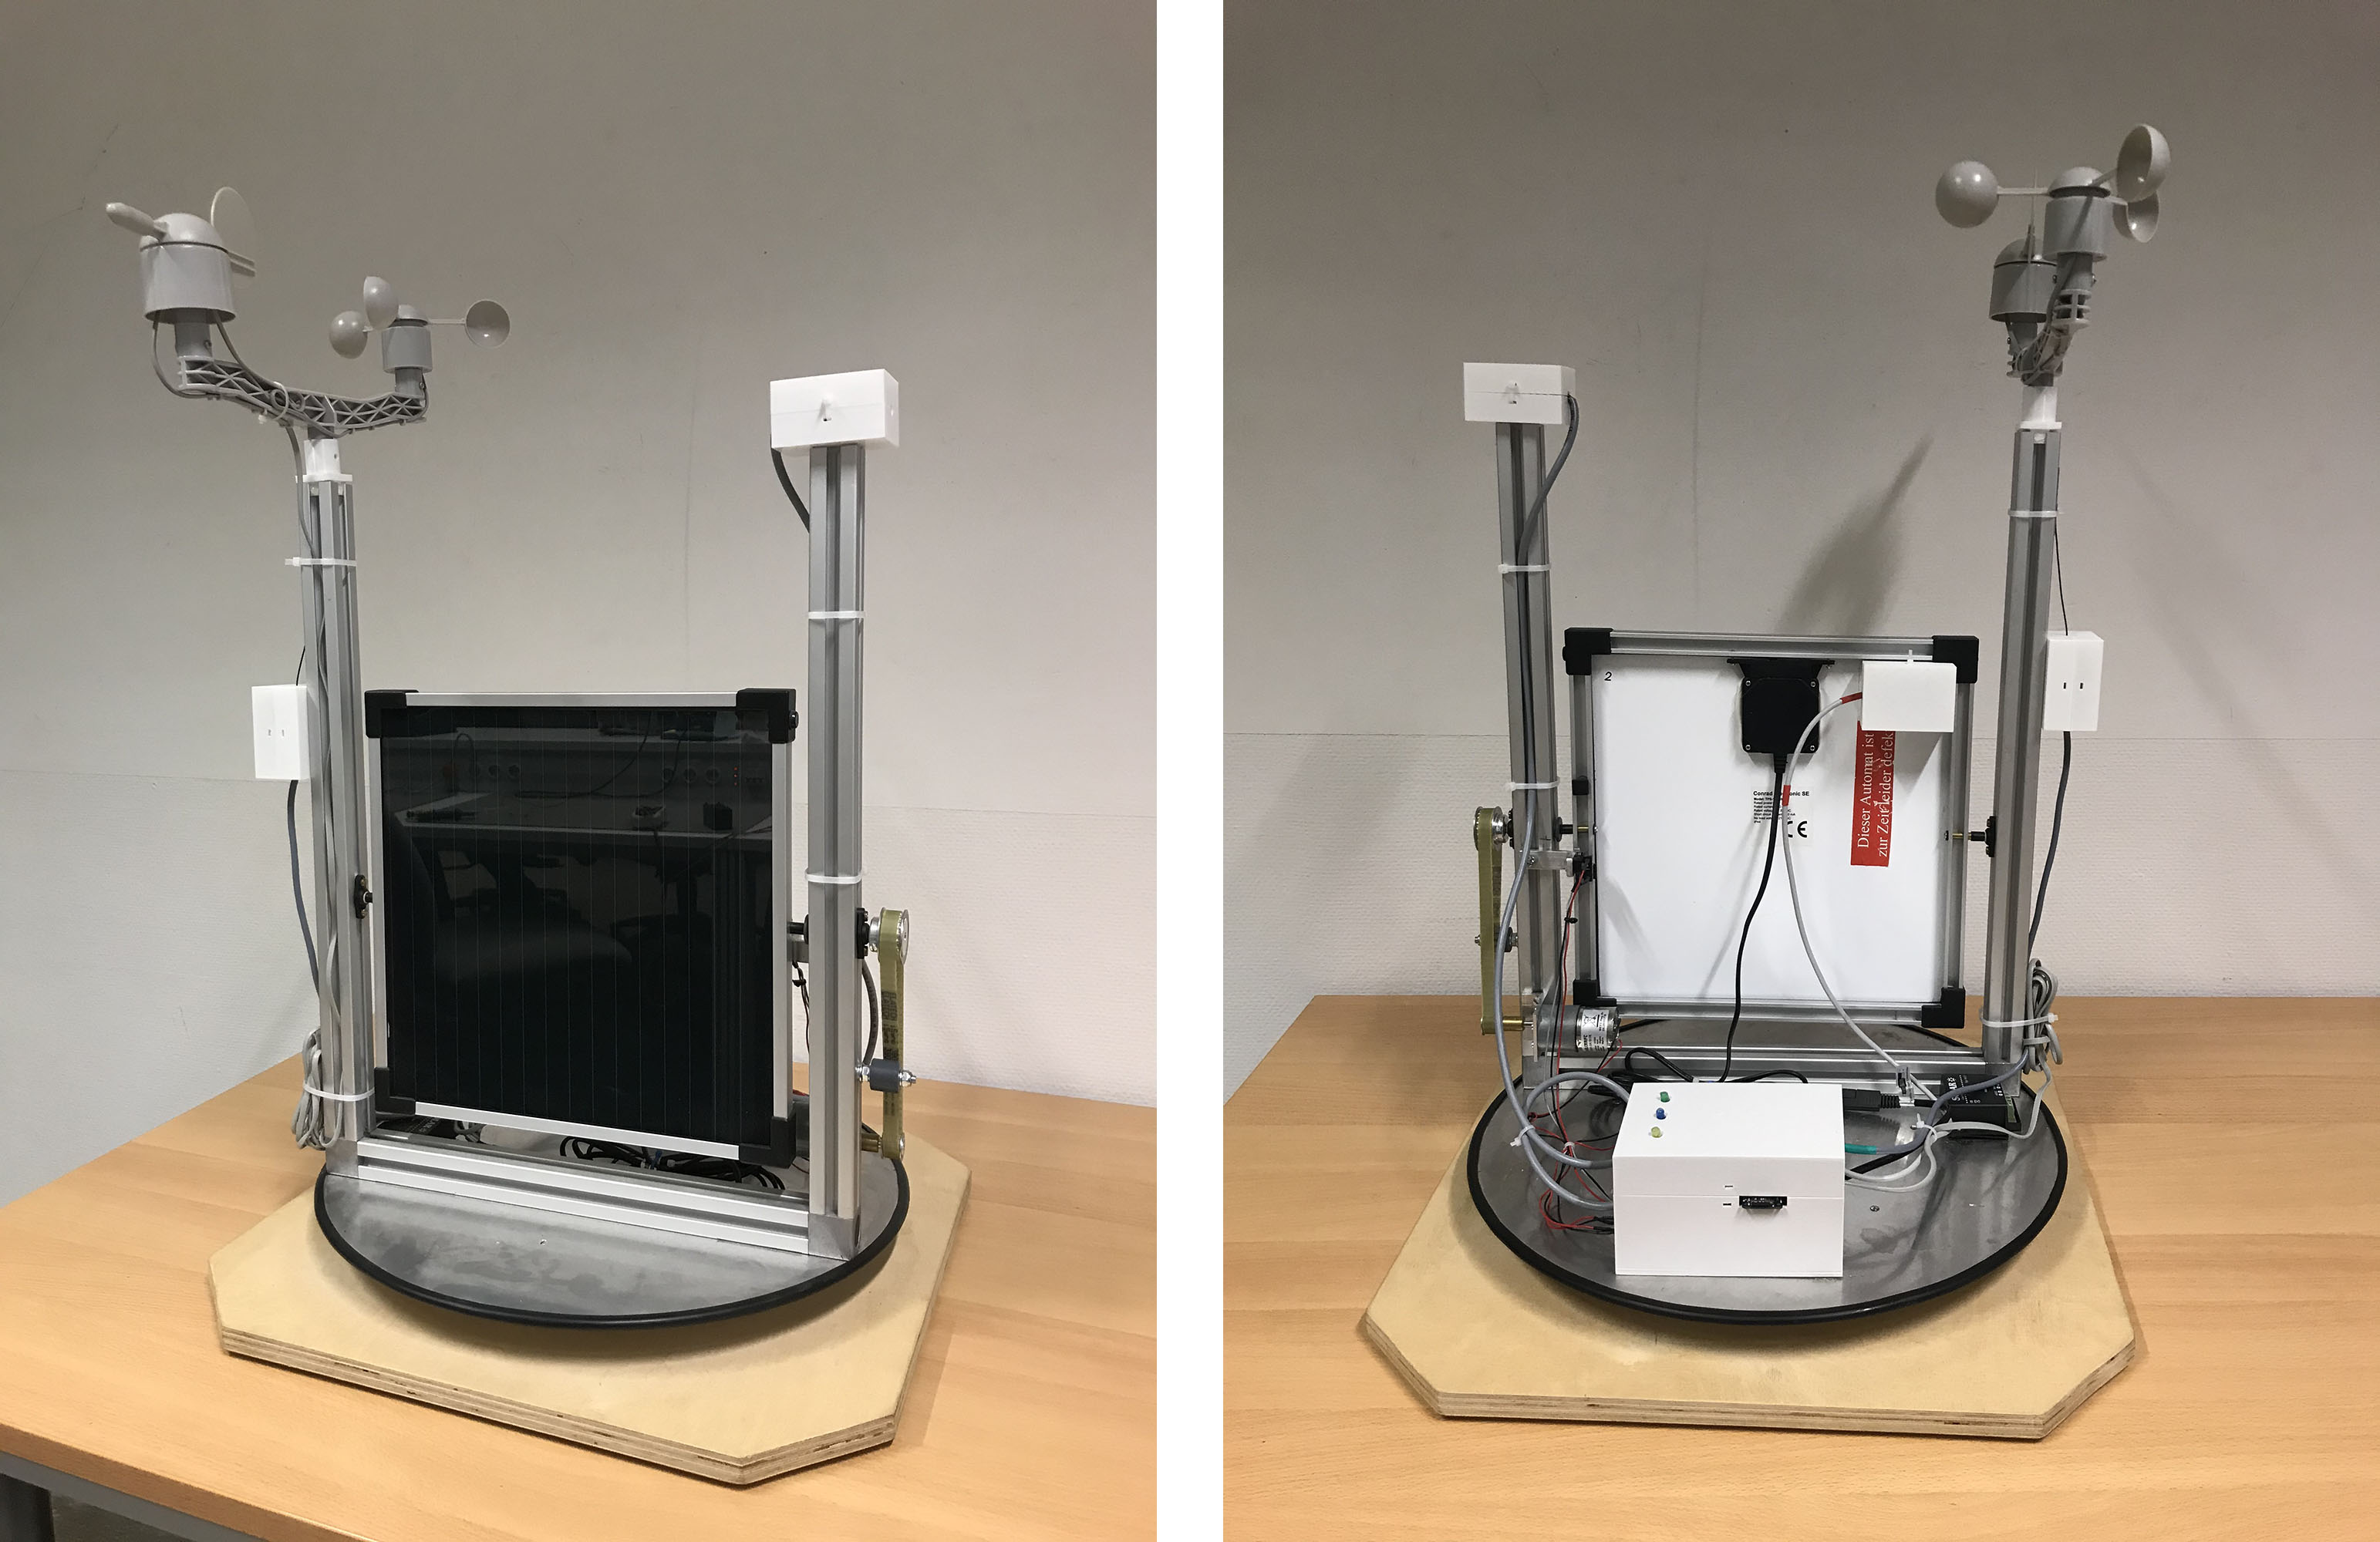
\includegraphics[width=0.8\textwidth]{./img/Wetterstaion_fertig1.jpg}
  \caption{Gegebener Aufbau der Wetterstation}\label{fig.Wetterstationfertig}
\end{figure}

In Abbildung \ref{fig.Wetterstationfertig} wird der fertige Aufbau der Wetterstation dargestellt. Die Anforderung der Erfassung von Temperatur, Luftdruck und -feuchte wird mit dem BME280, der im Hauptgehäuse platziert ist, umgesetzt. Für die Erfassung von Windrichtung und -geschwindigkeit konnte ein neues Anemometer gefunden und implementiert werden.

Im Hauptgehäuse ließen sich Mikrokontroller, Platinen und Sensoren sinnvoll unterbringen (Abbildung \ref{fig.hauptgehauese}). Die Wasserfestigkeit des Aufbaus konnte leider mit den verfügbaren Mitteln in der vorgegebenen Zeit nicht erreicht werden. Das verwendete 3D-Druck-Material ist nicht für einen abgedichteten Aufbau geeignet. 


\begin{figure}[H]
  \centering
  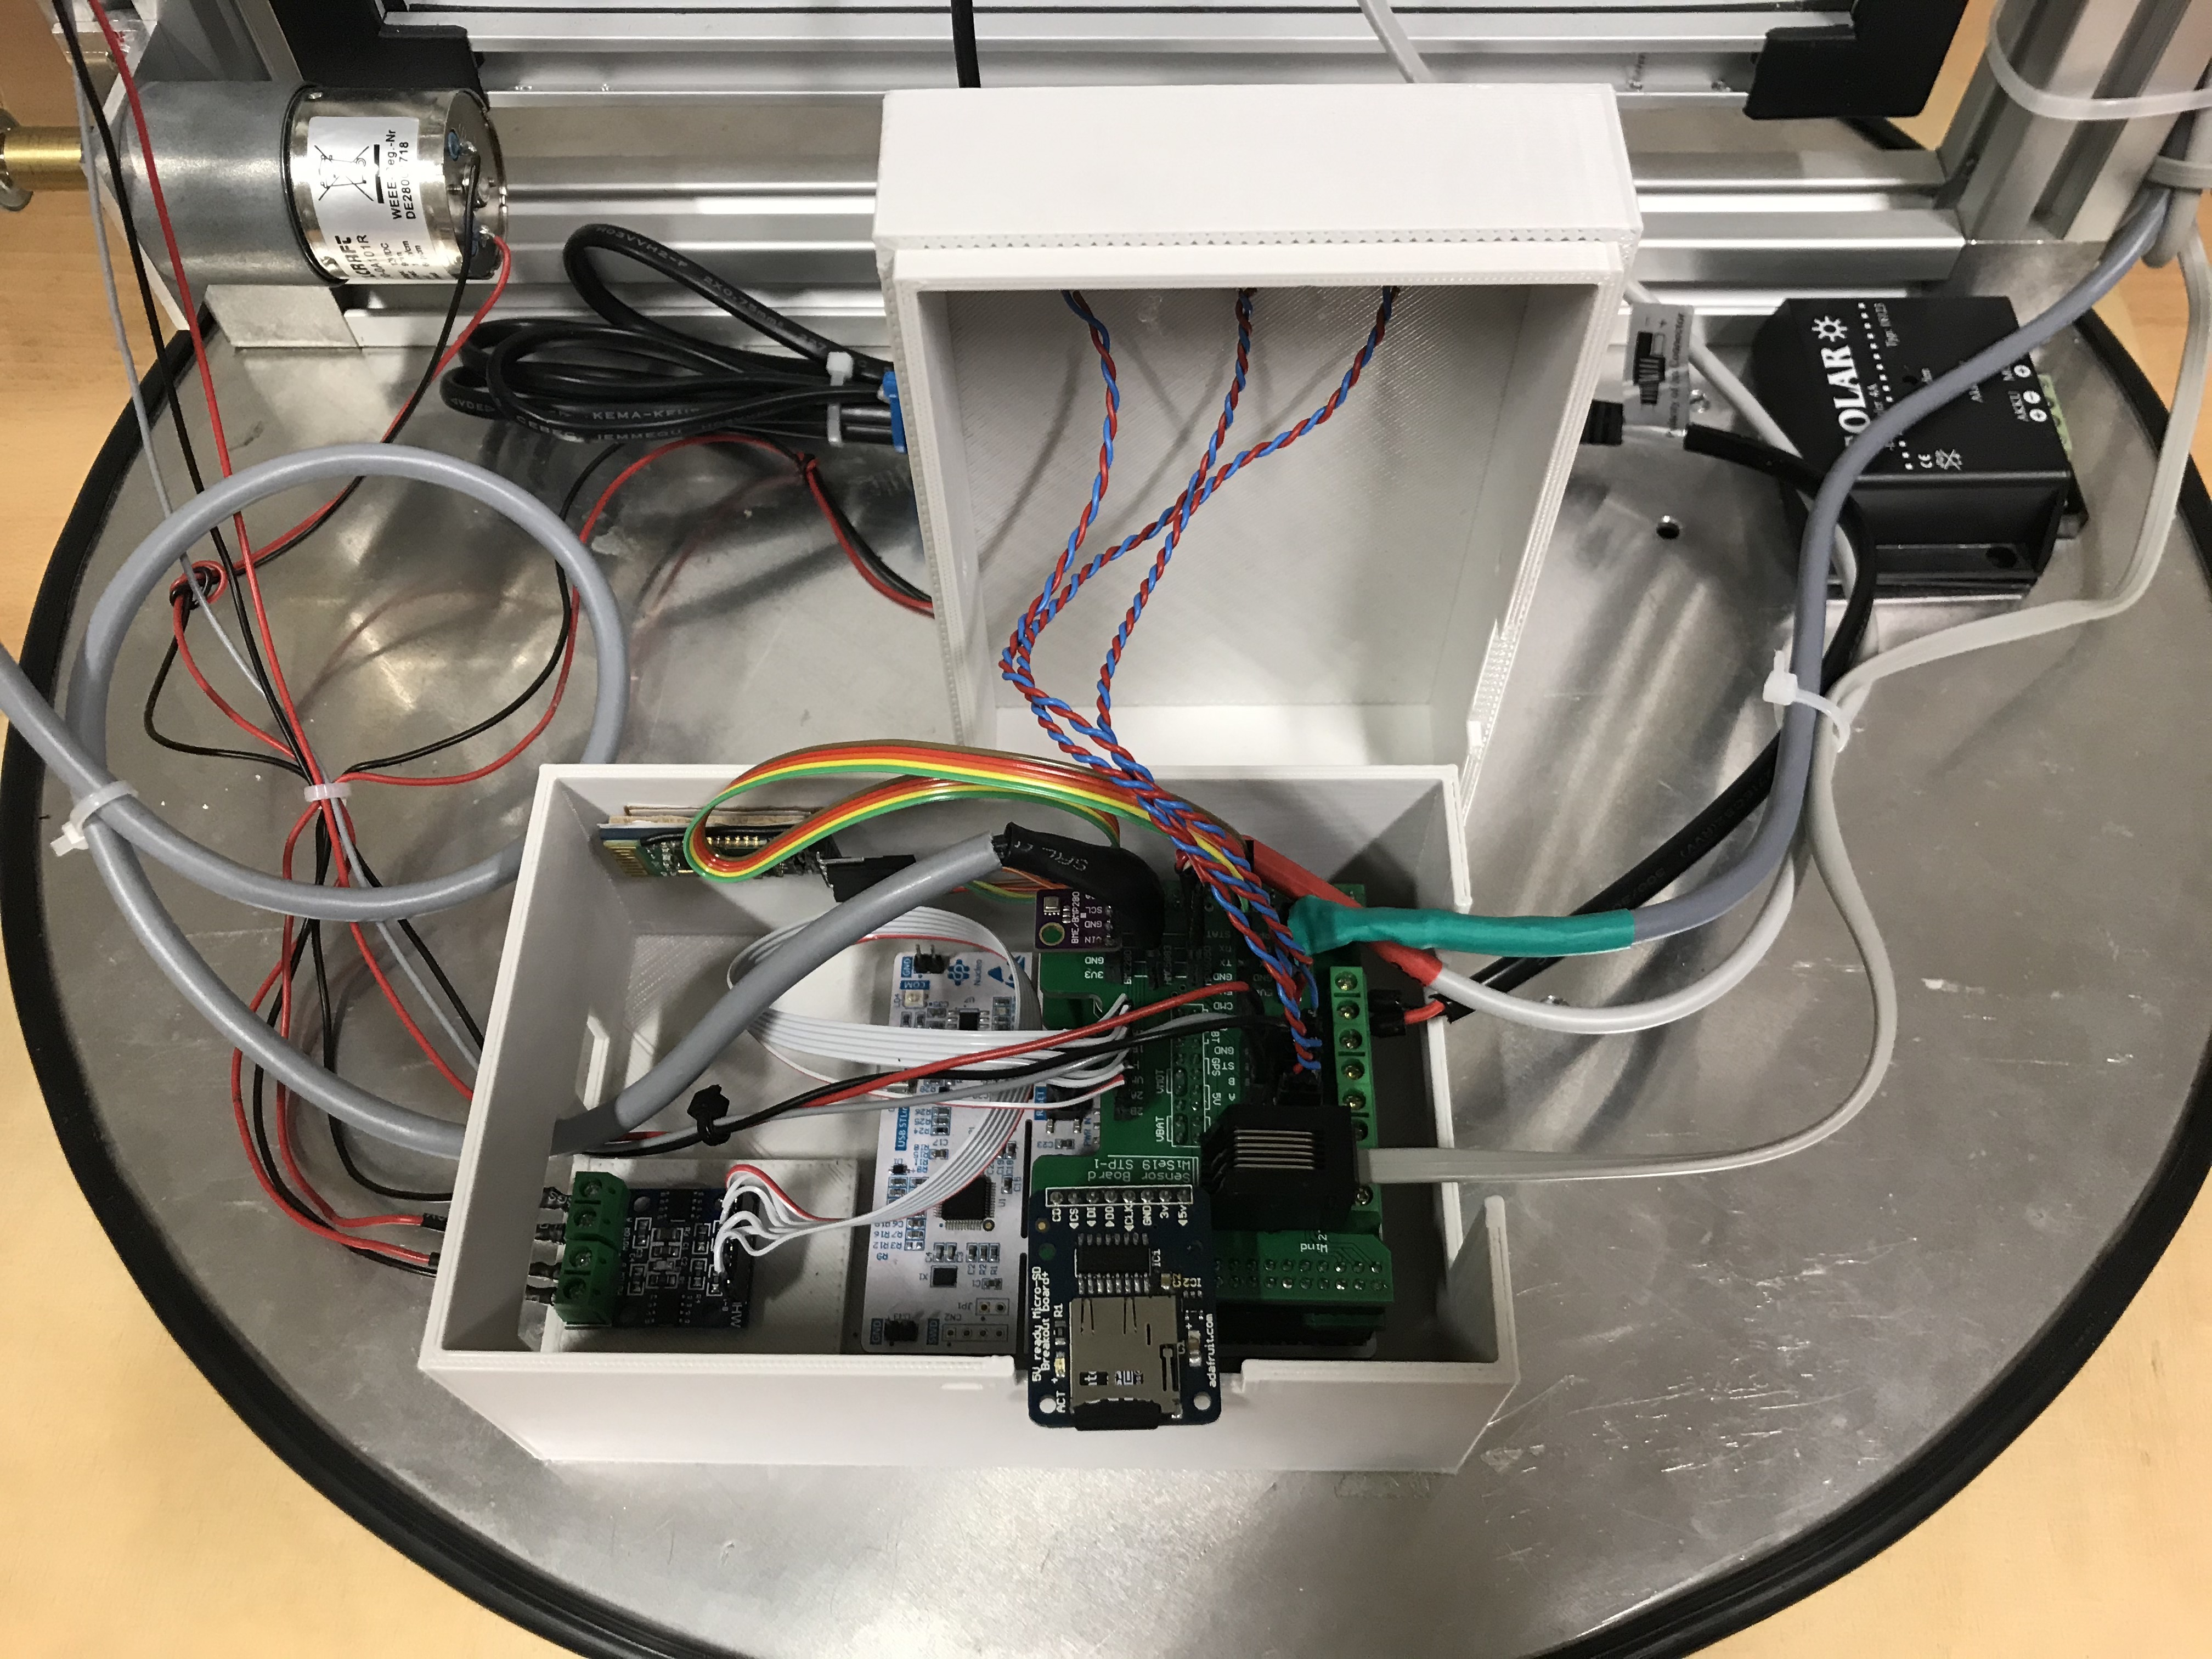
\includegraphics[width=0.7\textwidth]{./img/Hauptgehauese.jpg}
  \caption{Blick in das Hauptgehäuse}\label{fig.hauptgehauese}
\end{figure}

Sowohl hardware- als auch softwareseitig wurden verschiedene Energiesparmaßnahmen implementiert. Die letztendliche Laufzeit müsste noch in einem Langzeittest ermittelt werden.

Grundlegend lässt sich sagen, dass alle gegebenen Anforderungen erfüllt wurden und sogar um eine zusätzliche Benutzeroberfläche zum Abrufen der gemessenen Werte erweitert.

%Wasserfestigkeit nicht erfüllt, grundlegend umreißen, welche Anforderungen wie erfüllt wurden, Bild von der fertigen Wetterstation

%%% Local Variables:
%%% mode: latex
%%% TeX-master: "../termpaper"
%%% End:
